\documentclass{CML_Seminar_Template}

\begin{document}

\maketitle{Interruptions in HCI and Boundary Management}{\ }

\author{Andreas Rayzik}
       {Matrikelnummer 1891837}
       {andreas.rayzik@stud.uni-bamberg.de}

\begin{abstract}
Short abstract, max. 200 words  (Helvetica 10; height 13 Pt; 24 Pt above and below paragraph, centred). Abstract, abstract, abstract, abstract, abstract, abstract, abstract, abstract, abstract, abstract, abstract, abstract, abstract, abstract, abstract, abstract, abstract, abstract, abstract, abstract, abstract, abstract, abstract, abstract, abstract, abstract, abstract, abstract, abstract, abstract, abstract, abstract, abstract, abstract, abstract, abstract, abstract, abstract, abstract, abstract, abstract, abstract, abstract, abstract, abstract, abstract. 
\end{abstract}

\vspace{24pt}

\section{Introduction}

Job areas with on-call service mark a very interesting example of a boundary in which the consequences for unwanted transitions are especially high. The influences of constant interruptibility on mental and cognitive state become obvious. A questionnaire in 2006 and 2010 among Finnish physicians found that sleeping problems and WIF (work interference with family) lead to high distress, low job satisfaction and low work ability. The number of active on-call hours is associated with higher levels of WIF, but not with sleeping problems.
\par
Another study lists symptoms for mental, cognitive and behavioural effects. Table 1 shows a selection of symptoms. The kind of symptoms and their substantial prevalence among workers in on-call service shows the severity of the effects.

\section{The domain of on-call service}

\begin{figure}[htb]
  \begin{center}
   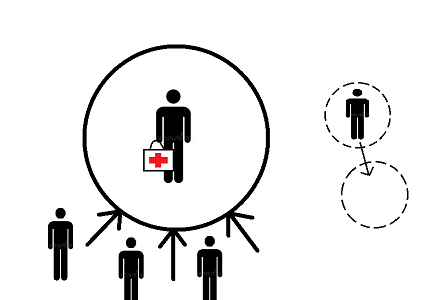
\includegraphics{Boundary_sketch_small.PNG}
  % \scalebox{.5}{\input{pager.jpg}}
  \end{center}
    \caption{\label{Boundary_sketch_fig}  Sketch depicting an on-call service worker in his domain and boundary. }
\end{figure}

\subsection{Effects on health}

In a 2006 study in Finland \cite[]{Lindfors2006}, researchers looked deeply into on-call stress and the effects among anaesthetists. Anaesthesia is a state of temporary induced loss of awareness or sensation. An anaesthetists is a physician trained in this field of medicine. In the questionnaire, an abundance of symptoms was asked about. A selection of a few of these symptoms was collected (cf. Table ~\ref{CML_Seminar_Template_tab1}). Reports of the symptom were compared between workers being currently on-call service or the day after and those on vacation for at least two weeks. It can be seen that for the selected symptoms, the report rates for on-call service are significantly higher. This is representative for the entirety of symptoms that was evaluated in the questionnaire. The symptoms involve mental, cognitive and behavioural kinds. They type of symptoms illustrate how severe the effects of on-call service are.


\begin{table}
\begin{center}
\begin{tabular}{ |c|c|c|} 
 \hline
 Symptom & On-call \% & On vacation \% \\
 \hline
 Tearfulness, depression & 23,2 & 3,3 \\
 \hline
 Memory disturbances & 45,8 & 9,5 \\
 \hline
 Need for alcohol & 30,5 & 18,4 \\
 \hline
 Need for sleeping medicine & 15,8 & 5,0 \\
 \hline
 Bulimia & 16,2 & 6,0 \\
 \hline
\end{tabular}
\end{center}
    \caption{\label{CML_Seminar_Template_tab1} Selected mental, cognitive and behavioural symptoms \cite[]{Lindfors2006}. }
\end{table}

\subsection{Boundary attributes}
The boundary of an on-call service exhibits an interesting combination of attributes. Boundary flexibility is defined by \cite[]{Piszczek2014} as the "Capacity of the boundary to be moved temporally or physically." Consequently, for the case of on-call service, the boundary flexibility has to be considered minimal. If we assume that no other worker would take the shift instead, the boundary must not be moved temporally. It must also not be moved physically, as the proximity to patients is critical and the distances to be covered need to be as short as possible. During an emergency, a time difference in minutes 
\par
Boundary permeability is defined by \cite[]{Hecht2009} as follows: "Reflects the extent to which an individual might be psychologically and/or behaviorally engaged in one domain, while physically located in another, or at times that are traditionally devoted to the other."
\par
Boundary thickness is defined by \cite[]{Ashforth2000} as the combination of boundary flexibility and boundary permeability. This means that the boundary thickness is debatable, since flexibility is minimal but permeability in contrast is high. When we separate both attributes by  



% \begin{quote}
% Quotations with a length of more than 40 words should be put in a separate paragraph (Times 10; % % height 13; 2 Pt above; 2 Pt below; 5 mm indenting)
% \end{quote}

% Refer to figures in the text (cf. Figure ~\ref{CML_Seminar_Template_fig1}).

% References in the text should have the format [Author Year]. Sources with one author should be referenced as \cite[]{Gro1995}; sources with two authors like this \cite[]{MaVa1984}, and sources with more than two authors like this \cite[]{Ham2002}; if you have the page numbers, indicate them like this \cite[p. 16]{Gro1995} or this for a range \cite[pp. 16-17]{Gro1995}. 

\section{How paging technology enables high availability}
Pagers are small devices that are designed to be dedicated to the one task of delivering text messages quickly and reliably. These messages are supposed to be short, concise and critical for the case of emergencies. Pagers are being used by hospitals, the police, energy distribution system operators and firefighters, to name some of the most important examples. Figure \ref{pager_fig1} shows an example of such a device. The interface elements on the front are very simple, with three arrow buttons for navigation and a power-on button. The display is a four-line alphanumeric monochrome display. The LCD has a back-light with adjustable contrast. It only displays the current date and time, and a message.
\par
Compared to a smartphone, the design is so much simpler and more efficient that the battery can be expected to last weeks instead of one or two days. The low-power CPU and the low-resolution monochrome display are the largest contributors to this feature. This is important in the case of a disaster, when there might be a power blackout and it is not possible to find a power outlet to charge a cellphone. The case of the device is sturdy and robust, so it can still function after being dropped from a moderate height. All of this contributes to a low-maintenance device, which on top of that can be quickly and inexpensively exchanged if it still gets lost or broken.

% TODO scale
\begin{figure}[htb]
  \begin{center}
   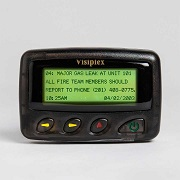
\includegraphics{pager_small.jpg}
  % \scalebox{.5}{\input{pager.jpg}}
  \end{center}
    \caption{\label{pager_fig1} An example of a paging device.}
\end{figure}

Paging technology operates in its own dedicated network. It has been proven to work during disasters, whereas the cellphone network tends to get overloaded and unreliable when many calls are being made. Paging provides encryption for data transport and over the air transmission. Compared to cellphone tower's signals, paging signals are more suitable to penetrate buildings. Additionally, they implement the so-called simulcast technology to combine signals for better reception.
\par
While smartphones always offer some form of option in their software to suppress alters or messages, pagers provide an alert that is inevitable and cannot be ignored. This is important because it takes a choice away from the user for the sake of reliability.
%TODO Trade-off between point-to-point and broadcast, maybe cite http://www.braddye.com/alerting.html
\par
Despite their old-fashioned and outdated appearance, the fact is that pagers are still in heavy use. They are relevant because they make a trade-off between complexity and reliability. Complexity, especially compared to smartphones, is reduced to a minimum in order to provide maximum availability. This availability leads to maximum reliability. The following section will explain how availability is related to interruptibility.

\subsection{Relation of availability and interruptibility}
To explain this relation, we need to give a more fine-grained definition of an interruption. In \cite[]{Fetter2018}, several subdefinitions of interruptions are collected from the literature and put into context very comprehensively. The figure \ref{interruptions_fig} of their work shall be taken to give an additional illustration of the hierarchy of definitions.

\begin{figure}[htb]
  \begin{center}
   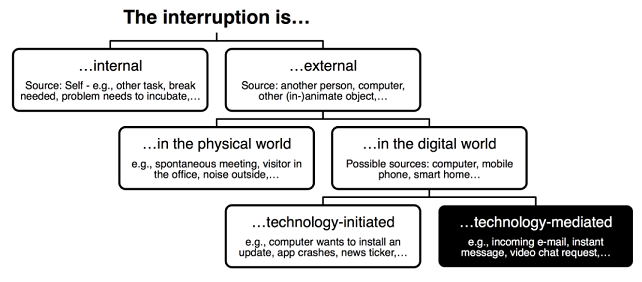
\includegraphics{interruption_definition_small.PNG}
  % \scalebox{.5}{\input{pager.jpg}}
  \end{center}
    \caption{\label{interruptions_fig}  Categorising interruptions based on the source and nature of the interruption. \cite[]{Fetter2018}}
\end{figure}

In the definitions, both the source and the nature of the interruption are being categorised. On the highest level, the authors distinguish between internal and external interruptions. Internal interruptions are all those which come from a subject's own thinking and needs. They can appear when a subject feels that he needs to draw its attention to another task or take a break. External interruptions on the other hand originate from the environment outside of the subject. Possible sources are not limited to persons. They can include for example a computer. External interruptions are being further broken down into those which happen in the physical world and those which take place in the digital world. Next, interruptions from the digital world are being split into technology-initiated and technology-mediated ones. At this point, a reference can be made back to paging technology and availability. Due to its design and its approach to minimize complexity, paging devices also reduce the technology-initiated kind of interruptions to a minimum while thereby leaving the greatest possible room for technology-mediated interruptions. In our case, the latter ones carry the information that is so critical in emergencies and so consequential when being missed. When we look at the examples that are given for technology-initiated interruptions, this becomes clearer.
\begin{itemize}
	\item A paging device generally is in no need for software updates. This is because its software has had decades of time to mature. On top of that, its simplicity makes it unlikely that bugs are being found. However, if there was a software update available, the pager would not regularly check for it the way a smartphone does. There is no functionality for over-the-air updates in paging. Since it cannot know when an update is available, it is impossible that the user is being prompted to install it. Instead, the user would have to manually check for the availability of an update on an external source like a website, download it and manually flash the pager's firmware with it. If there is no interface (e.g. USB) on the device to provide the user with this opportunity, he needs to rely on the device vendor to update its future products with the new software.
	\item The matured and simple software is also the reason why it is unlikely that it crashes on the pager. During its high amount of hours of operation on thousands of devices which all run the same software, potential bugs in the software would have with a high probability already lead to crashes. These crashes would have been likely lead to complains by the user and been investigated by the device vendor.
	\item The news ticker example does not apply to our case either. Paging devices are designed for one single purpose. A news ticker in the sense that general, informative news are being provided instead of critical ones would distract the user from this purpose. 
\end{itemize}

\subsection{Signalling availability in Life Domain after long periods of unavailability}
To avoid confusion, it has to be pointed out that in the previous sections, availability described the state of being able to receive interruptions in the work domain. Now, we would like to refer to being available in the life domain instead. After a long on-call working shift with maximum unavailability to the life domain, a worker might wish to balance this period with being highly available in the period afterwards. As has been discussed, the unavailability during the working hours contributes to a considerable amount of stress, that is expressed in an abundance of symptoms. A balance could help alleviate these symptoms. To take full advantage of his availability in the life domain, a worker needs to signal this state to his social environment. The signal needs to inform not only about the state of being technically reachable but the state of explicit availability. This way, communications can be initiated from both sides instead of originating from the worker only.
\par
As \cite[]{Fetter2018} explain, this can impose a challenge since there is a bias of signalling unavailability instead of availability in devices and software. Examples for this in smartphones are a Do-not-disturb mode or the Airplane mode, which is often being used for the same purpose. In text communication, there are typically the features of blocking another user, muting a contact's chat or a group chat, as well as disabling read confirmations. The latter one is being used to lessen the pressure of being expected to answer soon after a message was confirmed to the sender as being read. In devices, the bias becomes most obvious when evaluating sensor development and related signal processing. Examples for this are using the microphone sensor to capture voice activity or analysing the data of an accelerometer sensor the determine the activity of running. Captured voice activity might be interpreted as holding a conversation with another person. Both states, conversation and running, would reasonably be used to signal unavailability. Sometimes, this is motivated by trying to design a smartphone software feature to save battery life. In the state of unavailability, it is acceptable for the device to poll for incoming messages less frequently, which saves battery life by using the communications (e.g. WiFi) interface less and drawing less power for radio signal sending.

\subsection{Implications of the unavailability signalling bias}
In the work of \cite[]{Birnholtz2010}, some of the negative implications of signalling unavailability are being explored. In this perspective, it is not about how users are forced to signal unavailability by the software's bias. It is about users who purposefully invent different strategies to do such thing in order to avoid unwanted conversations or meetings. Nevertheless, these strategies begin to carry many negative associations for the user whose communication or approaching efforts are being rejected. Without a counterweight that also enables users to sometimes signal explicit availability instead, these negative associations become amplified.
In the paper, an experiment with 194 US students as participants is described. The authors wanted to find out how the users find ways of deceptive texting to avoid unwanted social interactions. The strategies were termed "butler lies", hinting at the role butlers used to employ for their boss. When 
undesired visitors requested to meet their boss, the butlers would tell them that he or she was busy when in fact the interaction was merely unwanted. Birnholtz et al. discovered three main strategies:
\begin{itemize}
	\item Temporal ambiguity: These were phrases like for example "sorry I just your text", hiding the fact that the text had actually been read long before. In the experiment, traditional SMS text messages were used which do not implement read confirmations. The users exploited this lack of information to have an excuse to not react or answer earlier to a message.
	\item Activity ambiguity: This term describes messages like for example "Eating now, can I call you later?" The stated activity was not the activity that the user was really pursuing at the time of typing the message. These kinds of texts were often used to delay a conversation, without risking impoliteness by cancelling the conversation altogether.
	\item Giving multiple options: In this strategy, the message sender was explaining that he was not yet sure whether to attend one of multiple events or go to one of several places. Leaving the possibility of a meeting open, the sender had actually already decided for himself against a meeting with the other person.
\end{itemize}


%\subsection*{Books:} 
%
%\cite[]{Ham2002, MaVa1984}
%
%\subsection*{Journals:}
%
%\cite[]{Gro1995}
%
%\subsection*{On-line Sources:} 
%
%\cite[]{Bal1994}
%
%\subsection*{Conference Proceedings:} 
%
%\cite[]{GrPr2003}
%
%\subsection*{Ph.D. and Master's theses:}
%
%\cite[]{Dou1996}
%
%\subsection*{Reports:} 
%
%\cite[]{BeMa1993}


%\section*{Acknowledgements}
%
%\begin{acknowledgements}
%Acknowledgements. 
%\end{acknowledgements}

\bibliography{CML_Seminar_Template}

\end{document}
